% LaTeX Article Template - customizing header and footer
\documentclass{article}

\newtheorem{thm}{Theorem}

% Set left margin - The default is 1 inch, so the following 
% command sets a 1.25-inch left margin.
\setlength{\oddsidemargin}{0.25in}

% Set width of the text - What is left will be the right margin.
% In this case, right margin is 8.5in - 1.25in - 6in = 1.25in.
\setlength{\textwidth}{6in}

% Set top margin - The default is 1 inch, so the following 
% command sets a 0.75-inch top margin.
\setlength{\topmargin}{-0.25in}

% Set height of the header
\setlength{\headheight}{0.3in}

% Set vertical distance between the header and the text
\setlength{\headsep}{0.2in}

% Set height of the text
\setlength{\textheight}{9in}

% Set vertical distance between the text and the
% bottom of footer
\setlength{\footskip}{0.1in}

% Set the beginning of a LaTeX document
\usepackage{multirow}
\usepackage{fullpage}
\usepackage{graphicx}
\usepackage{amsthm}
\usepackage{amssymb}
\usepackage{url}
\usepackage{color}
\usepackage{algpseudocode}
\usepackage{listings}
\graphicspath{%
    {converted_graphics/}% inserted by PCTeX
    {/}% inserted by PCTeX
}
%%%%%%%%%%%%%%%%%%%%%%%%%%%%%




\begin{document}\title{Midterm\\ Computer Science \\ Fall 2015\\ B565}         % Enter your title between curly braces
\author{Ganesh Nagarajan\\gnagaraj@indiana.edu\\ Sunday, October 25, 9:00 p.m.}        % Enter your name between curly braces
\date{\today}          % Enter your date or \today between curly braces
\maketitle


% Redefine "plain" pagestyle
\makeatother     % `@' is restored as a "non-letter" character



% Set to use the "plain" pagestyle
\pagestyle{plain}
\section*{Solutions}
All the work herein is solely mine.\\
Inorder to solve the given problem, following were the libraries and tools that contributed significantly.\\

\begin{tabular}{|c|c|c|} \hline
$Tool/Library$ & $Version$ & $Acknowledgement \: to$ \\ \hline 
R & 3.2.2 & CRAN \\
R Studio & 0.99.446 & RStudio, Inc\\
MySql Database & 5.6.26 & Oracle, Inc\\
Talend Open Studio for Data Integration & 6.0.0 & Talend, Inc\\
RMySql & 0.10.6 & Jeroen Ooms et.al\\
cluster & 2.03 & Martin Maechler et.al\\
corrplot & 0.73 & Taiyun Wei\\
arules & 1.2-1 & Michael Hahsler et.al\\
arulesViz & 1.0-4 & Michael Hahsler et.al \\
e1071 & 1.6-7 & David Meyer et.al \\
ggplot2 & 1.0.1 & Hadley Wickham \\
\hline
\end{tabular}
\section*{Application: Solutions}
\subsection*{Problem Statement}
An interview was done with  Filmflix.com to understand their business requirements for using data to their competitive advantage.
There were key discussing about using data mining algorithms to understand their given data. A database schema of their operational systems were given for analysis.
\subsection{Data Preparation}
The Given data is in its operational or OLTP form, and hence cannot be used for any analysis. This data must be transformed to a suitable form for analysis. For this purpose, MySql database is used for data persistence and Talend ETL tool is used for data integration. Following were the data cleaning activities done to process the data.
\begin{enumerate}
\item Data Creation
\begin{enumerate}
\item The given data was reproduced in R and is converted to data frames.
\item Once the suitable column names are given, this data frame is exported to CSV.
\begin{lstlisting}[language=R]
#This program creates the CSV files for data ingestion. 
#The data frame is converted to an CSV file, which is loaded 
#to database using ETL 
Genere<-c("Romance","Science  Fiction","Horror","Comedy","Drama","Action",
          "Documentary","Classic")
Code<-c("r","s","h","c","d","a","o","l")
DC<-as.data.frame(cbind(Genere,Code))

mv1<-c("1","r","s",NA,NA)
mv2<-c("2","o","l","a",NA)
mv3<-c("3","c","d","h",NA)
mv4<-c("4","s","l","o","a")
mv5<-c("5","a","d","r",NA)
mv6<-c("6","d","h","c",NA)
mv7<-c("7","a","d","c","o")
mv8<-c("8","h","l","r",NA)
mv9<-c("9","s","d",NA,NA)
mv10<-c("10","c","r",NA,NA)
MIDG<-as.data.frame(rbind(mv1,mv2,mv3,mv4,mv5,mv6,mv7,mv8,mv9,mv10))
colnames(MIDG)<-c("Mv_ID","G1","G2","G3","G4")

C1<-c("CID1","CID2","CID3","CID4","CID5","CID6","CID7","CID8","CID9","CID10",
      "CID11","CID12","CID13","CID14")
C2<-c(1,4,7,2,4,3,1,5,10,2,1,3,8,5)
C3<-c(3,1,8,NA,8,9,2,4,1,4,10,5,1,2)
C4<-c(5,2,1,NA,10,10,3,9,2,3,8,1,7,8)
C5<-c(5,3,NA,NA,NA,1,NA,5,23,7,NA,2,NA,NA)
C6<-c(10,NA,NA,NA,NA,NA,NA,NA,NA,9,NA,NA,NA,NA)
c7<-c(8,NA,NA,NA,NA,NA,NA,NA,NA,NA,NA,NA,NA,NA)
CIDM<-as.data.frame(cbind(C1,C2,C3,C4,C5,C6,c7))

write.csv(CIDM,"CIDM.csv")
write.csv(DC,"DC.csv")
write.csv(MIDG,"MIDG.csv")
\end{lstlisting}
\item Once the data is available as CSVs, workflow jobs were created to copy this data to the MySQL database.
Since Talend is an metadata based orchestration tool, we don't have to work with any data, rather only with the metadata.
This metadata has been used to define the table schemas in the target database. Following is the screen shot of the workflows created.\\ \\
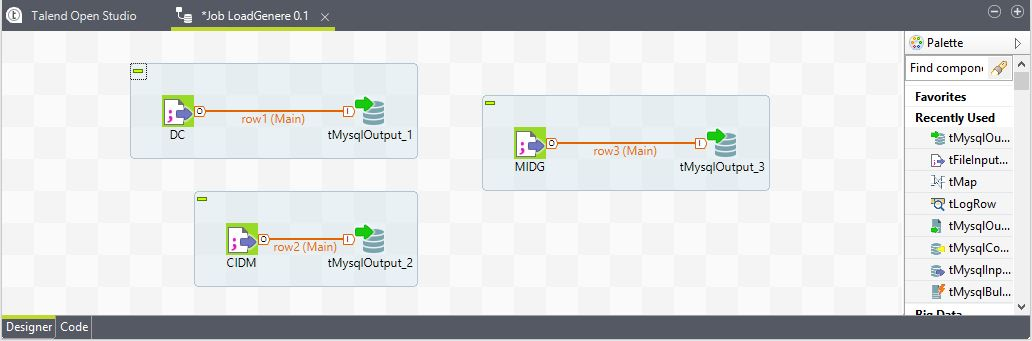
\includegraphics[scale=0.5]{ETl.JPG}\\
A nifty feature of the tool is the option $create \: table \: if \: it \: doesn't \: exist$. Hence once the tool finds there is no table, it creates the table with the metadata that was designed in the tool's repository.\\ \\
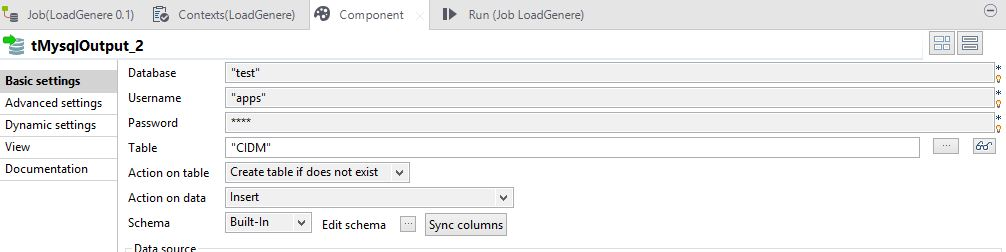
\includegraphics[scale=0.5]{ifexists.JPG}\\
An export of this schema is attached with this homework if its needs to be reproduced.
The schema name is test, no password, i.e blank password. In all connections, localhost is used to query the database.
\end{enumerate}
\item Data Transformation
\begin{enumerate}
\item Since we have the data available for querying, now we have to transform the data for queries.\\
Data Mining algorithms require specific format for data input. Eg, Clustering algorithms require features as columns.\\
Hence using SQL, several temporary tables were created, several aggregations were performed to make the final data ie customers as rows and Genere / Movies seen as columns.\\
A sample code is given here. However, the entire script is attached with this homework.
\lstinputlisting[language=SQL,firstline=1,lastline=53]{transform_data.sql}
A screenshot of a sample table is given below.\\
This table aggregates the views in genere by customer. Similarly other table, aggregation the views of film by customer is also created with other supporting tables.\\ \\
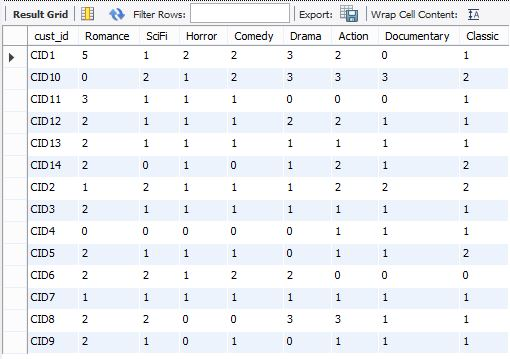
\includegraphics[scale=1]{sql_rs1.JPG}\\
\end{enumerate}
\end{enumerate}
\subsection*{Exploratory Data Analysis}
Since we have the data now, in a format that can be used for analysis, visualizing data will help to understand more about the data. This helps the feature engineering process of data mining if its required. RSQL package is used to connect R to the MySQL database and the visualizations are plotted through ggplot2.\\
\begin{enumerate}
\item Plot of the entire genre vs customers are as follows.\\
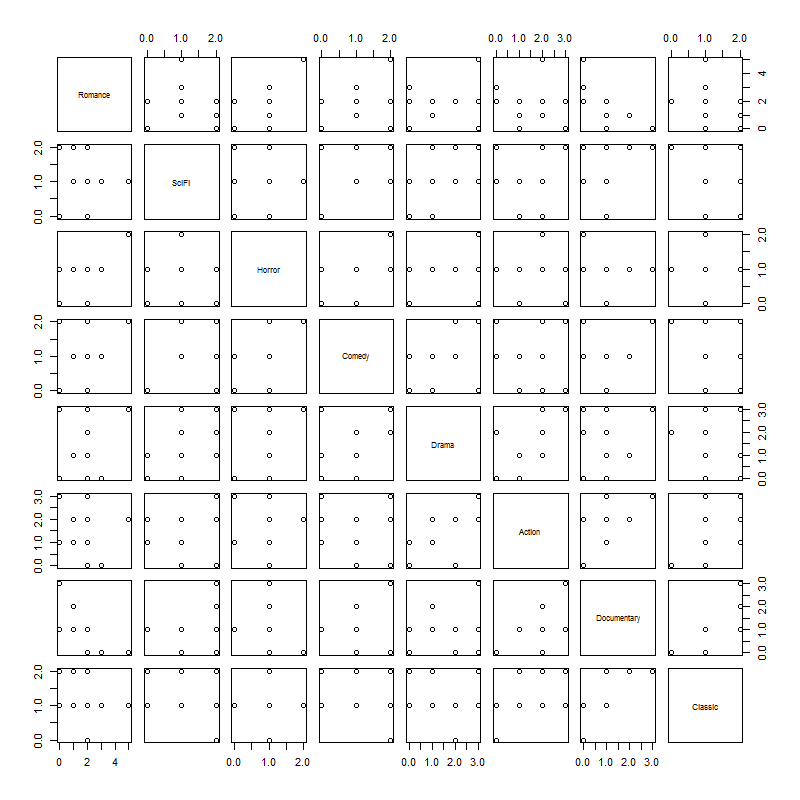
\includegraphics[scale=0.5]{EDA1.png}\\
It can be visually seen that there are some repeating patterns in the dataset. Hence this can be studied further for dimensional reduction perspective.
\item Since this is a small dataset, we can visualize the entire dataset. Following graphic segregates the views of all customers by genere. Eg, Customer 1 has seen the highest movies in Romance Genre!\\
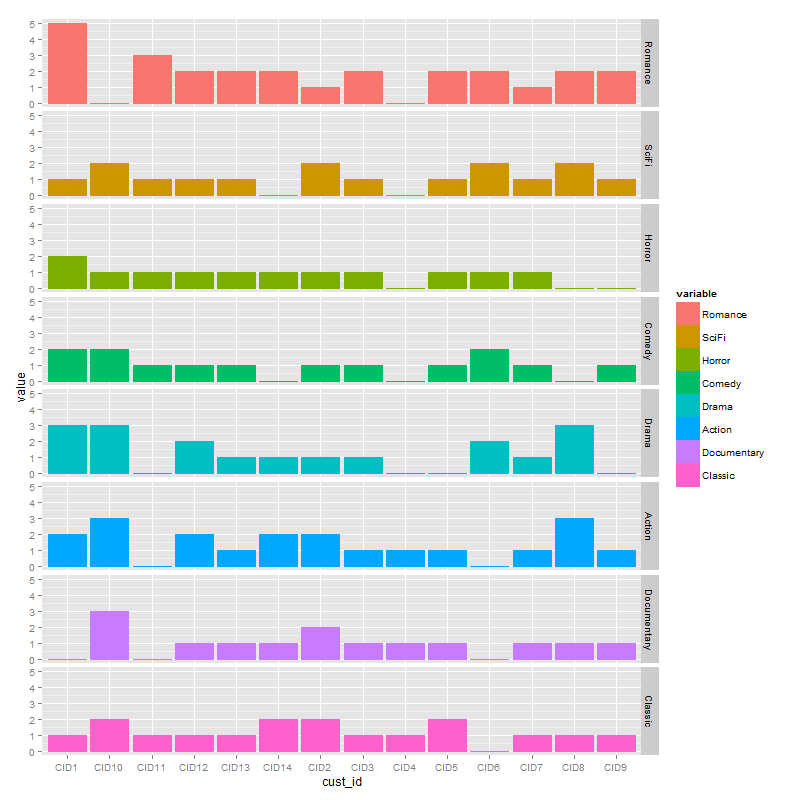
\includegraphics[scale=0.5]{EDA2.png}\\
\item When taking about promotions, it is important to understand what movies and generes are popular. Following visuals capture the popular generes and films by number of views.\\
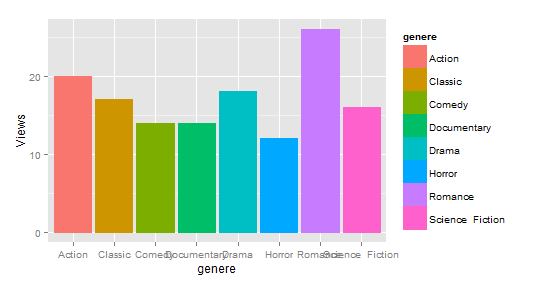
\includegraphics[scale=0.5]{EDA3.png}\\
It seems the most watched genre is Romance!\\
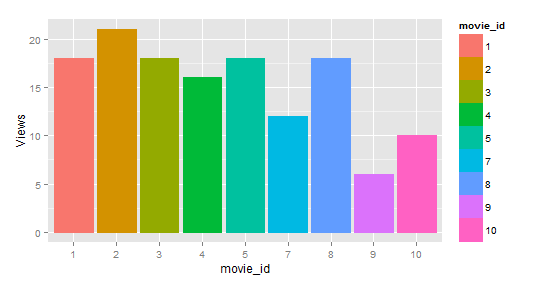
\includegraphics[scale=0.5]{EDA4.png}\\
And movie 2 is the most watched movie of all times!\\
These popular items will help us in promotion of the films.
\end{enumerate}
\subsection{K-Means for Segmentation}
Businesses would like to do segmentation of its customers by purchase power, buying patterns etc, FilmFlix, being an internet company, requires to segment the group both by genre aswell as the common films seen.\\
\begin{enumerate}
\item Determination of K for k-Means\\
Optimal k ensures the interpretability of that cluster. Inorder to identify k, a function was written in R, which calculates the sum of inter block distances between the blocs. A balance has to be attained between the number of k and the minimal inter block distance. As the number of block approaches number of elements, it is indeed that the intra block distance reduces, however now each block is an element, hence would not explain anything. Hence a key is to choose a k, which is in the knee point of the curve.\\
A four iteration trial was made to training dataset, and it is seen that in all 4 curves, three remains to be the most optimal point. Hence 3 is chosen as k.\\
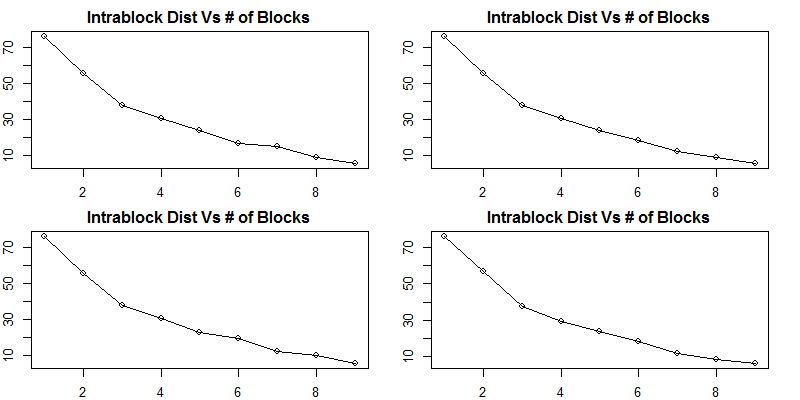
\includegraphics[scale=0.5]{kdeterminationbygenere.png}\\
\item Implementation for Genre\\
K-Means was run to this setting, with input as a dataframe consisting customers as rows and Genre as columns.\\
Following is the code,\\
\lstinputlisting[language=R]{kmeans.R}
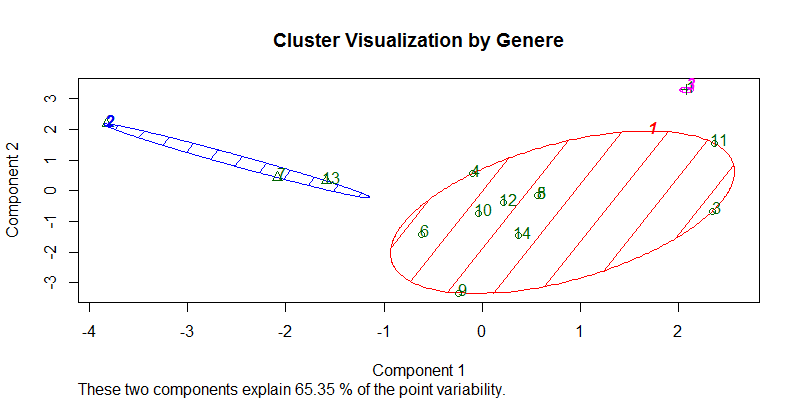
\includegraphics[scale=0.5]{clustervisualbygenere.png}\\
Cluster package was used to visualize the cluster. This was run several times and the most consistent cluster is shown above.\\
When this cluster was analyzed,\\
Cluster 1 : Represents Drama, Action, Documentary and Classics. Most of the customers in this segment see these above said genre.\\
Cluster 3 : Represents customers who have seen maximum of Romance films.\\
Cluster 2 : Represents a wide spread of Genere. Most of these customers have seen atleast a film in every Genre.\\
\item Implementation of K-Means to customers who have seen similar films.
\begin{enumerate}
\item Determination of K \\
As described above, a inter block distance vs clusters was plotted for this dataset. This hints that there could be three clusters in this dataset also.\\
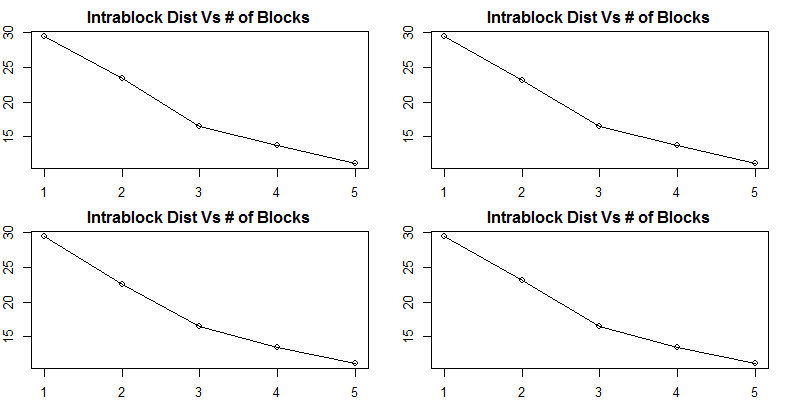
\includegraphics[scale=0.5]{kdeterminationbymovie.png}\\
\item The structure of this dataset is, customers in rows and Movies in columns. The cross numbers represent the views of the movie.
\item In this dataset, there were few observations: \\
\begin{enumerate}
\item No one has seen movie 6. Hence can be removed from the dataset.
\item A correlation matrix of the dataset brings that correlation of movie 8 and 9 are 1, ie everyone who has seen movie 8 have seen movie 9!.\\ This is an interesting data, An offer of 20 percent can be given to anyone who are seeing both the movies!\\
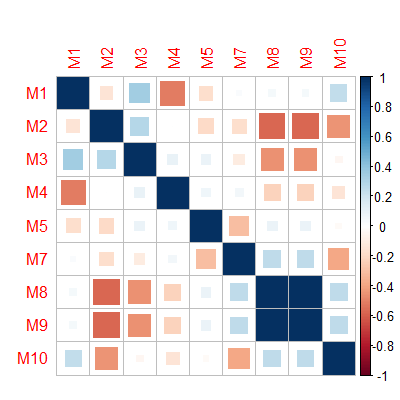
\includegraphics[scale=0.5]{movie_df_corrmatrix_asquare.png}
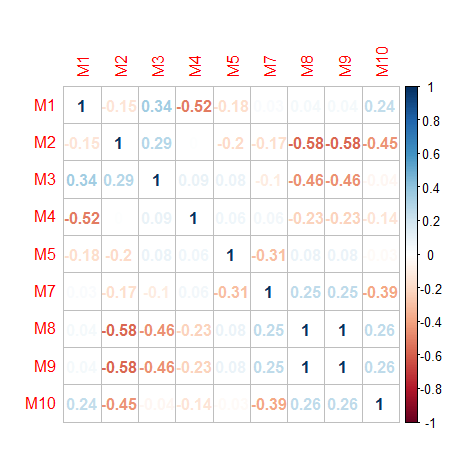
\includegraphics[scale=0.5]{movie_cor_numbers.png}\\
Also from computational perspective, we can either of the column, because these two represent the same features.
\item There were few erroneous data, E.g there is no movie with id 23. Hence this data was removed.
\end{enumerate}
\item K-Means for Movie Dataset\\
Now since the data is already prepared, and k=3 is determined as optimal number of clusters, K-Means was done. Following is the visualization of that cluster.\\
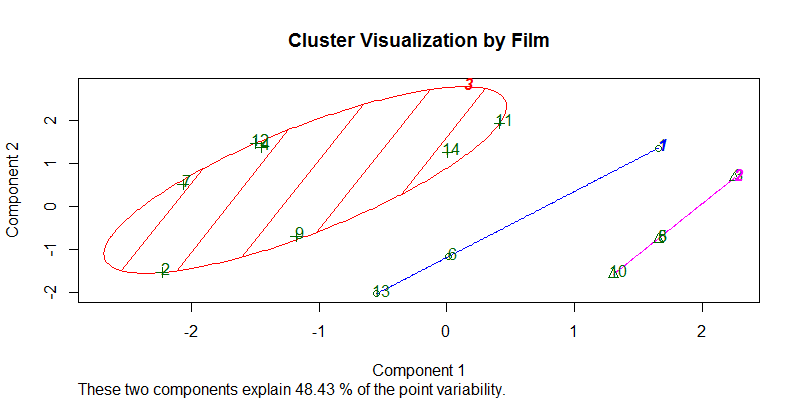
\includegraphics[scale=0.5]{clustervisualbyfilm.png}\\
This figure is self explanatory,\\
Cluster 1 : 13,6,1 customers have similar patterns.\\
Cluster 2 : 10,8,3 customers have similar patterns.\\
Cluster 3 : Rest all customers have similar patterns.
\end{enumerate}
\end{enumerate}
\subsection*{Association Rules}
\begin{enumerate}
\item Association rules in current application context is used to find what genre/movies are bring watched together.\\ The library used for this is Apriori algorithm and AprioriViz library is used for visualization of these rules.
\begin{enumerate}
\item Apriori by Genre
\begin{enumerate}
\item: Data Preparation \\
Since Apriori algorithm does not worry about features as such, however is interested in transactions, following is a sample datastructure that was used for apriori.
\begin{verbatim}
genere_df
    cust_id movie_id           genere
1      CID1        1          Romance
2      CID1        1 Science  Fiction
3      CID1        3           Horror
4      CID1        3            Drama
5      CID1        3           Comedy
6      CID1        5           Action
7      CID1        5          Romance
.....
17    CID10        2          Classic
18    CID10        2           Action
\end{verbatim}
i.e, every customer is considered as an transaction. This data is queried from the database and is written to a CSV files.\\
These CSV files are then manually opened and the quotes are deleted. This processed file is then directly imported as transactions deleting the duplicate entries.\\
\item The complete code is as follows,\\
The parameters used are, supp=0.7,conf=1
\lstinputlisting[language=R]{apriori.R}
\begin{verbatim}
inspect(ru_genere)
   lhs                          rhs                support   confidence lift    
1  {Documentary}             => {Action}           0.7857143 1          1.166667
2  {Documentary}             => {Classic}          0.7857143 1          1.076923
3  {Comedy}                  => {Science  Fiction} 0.7857143 1          1.166667
4  {Action}                  => {Classic}          0.8571429 1          1.076923
5  {Action,Documentary}      => {Classic}          0.7857143 1          1.076923
6  {Classic,Documentary}     => {Action}           0.7857143 1          1.166667
7  {Comedy,Horror}           => {Science  Fiction} 0.7142857 1          1.166667
8  {Horror,Science  Fiction} => {Comedy}           0.7142857 1          1.272727
9  {Comedy,Romance}          => {Science  Fiction} 0.7142857 1          1.166667
10 {Classic,Comedy}          => {Science  Fiction} 0.7142857 1          1.166667
11 {Action,Romance}          => {Classic}          0.7142857 1          1.076923
12 {Action,Science  Fiction} => {Classic}          0.7142857 1          1.076923
\end{verbatim}
\item Visualization and Interpretation:\\
The below graphics are beautiful to interpret the association rules in graphical form, especially the graph chart.\\
It can be seen that people who watch {Action,Documentary}, always see {Classic}.\\
Also people who see {Classic,Documentary} always see {Action}.\\
Hence there can be an discount of 25 percent when all movies of one in three genre are bought together!\\
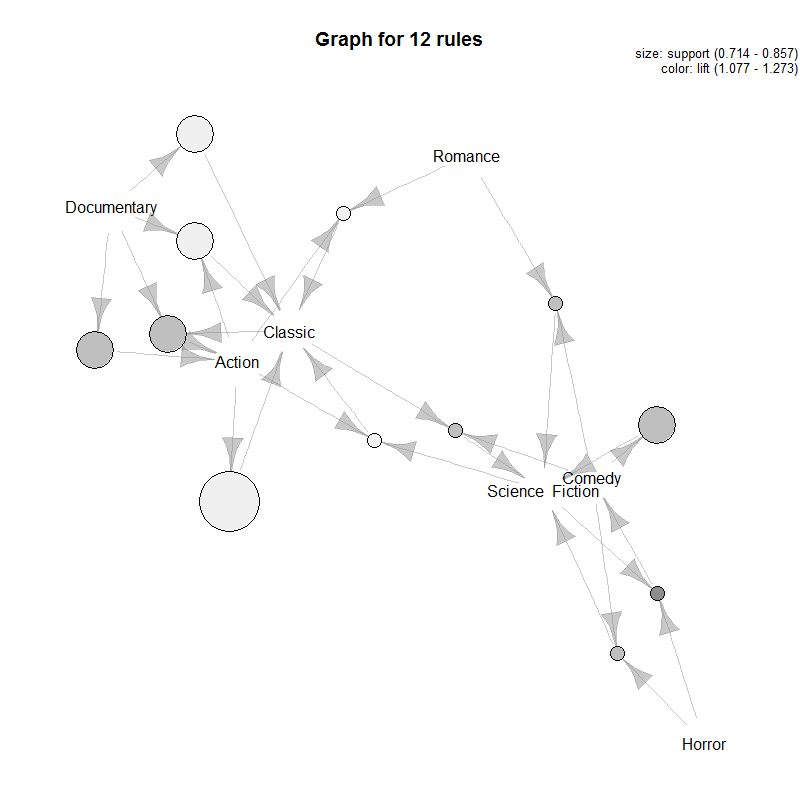
\includegraphics[scale=0.5]{association_genere_1.png}\\
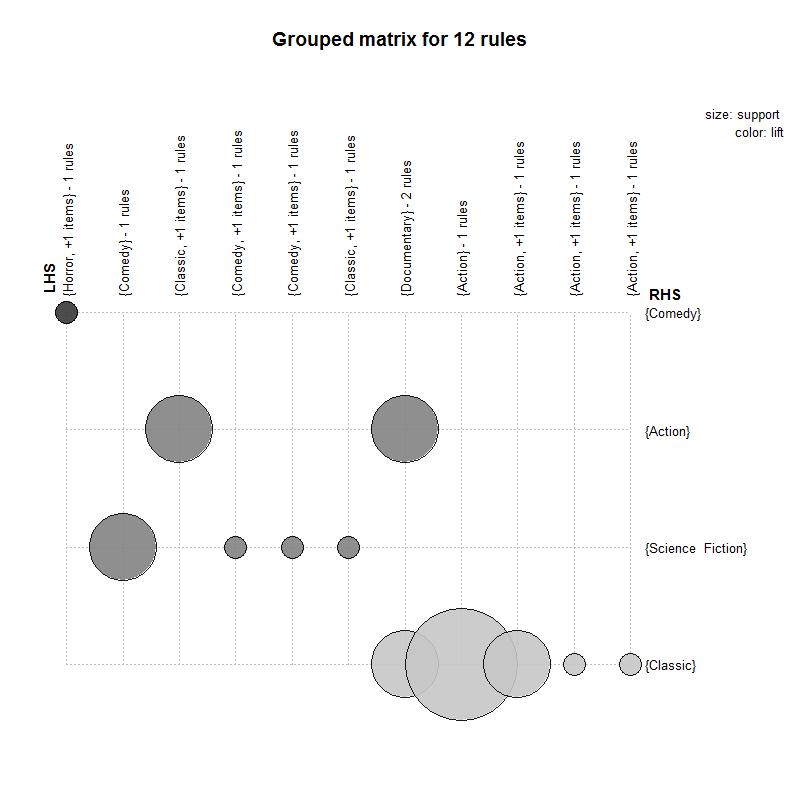
\includegraphics[scale=0.5]{association_genere_2.png}\\
\end{enumerate}
\end{enumerate}
\item Visualizing for Films:\\
\begin{enumerate}
\item Similar to the data processed for above method, the transnational nature of the data presented for film assocation is as follows.
\begin{verbatim}
movie_df
   cust_id movie_id
1     CID1        3
2     CID1        5
3     CID1        5
4     CID1       10
....
7    CID10        3
8    CID10        7
9    CID10        9
\end{verbatim}
Same as above method, Customer id is the transaction number here.
\item Implementation:\\
Apriori algorithm was run with supp=0.2,conf=0.5 parameters and following is the output.
\begin{verbatim}
lhs      rhs  support   confidence lift     
1  {}    => {2}  0.5000000 0.5000000  1.0000000
2  {}    => {1}  0.6428571 0.6428571  1.0000000
3  {10}  => {8}  0.2142857 0.6000000  1.4000000
4  {8}   => {10} 0.2142857 0.5000000  1.4000000
5  {10}  => {1}  0.2857143 0.8000000  1.2444444
6  {8}   => {1}  0.2857143 0.6666667  1.0370370
7  {2}   => {3}  0.2857143 0.5714286  1.3333333
8  {3}   => {2}  0.2857143 0.6666667  1.3333333
9  {2}   => {1}  0.2857143 0.5714286  0.8888889
10 {3}   => {1}  0.3571429 0.8333333  1.2962963
11 {1}   => {3}  0.3571429 0.5555556  1.2962963
12 {2,3} => {1}  0.2142857 0.7500000  1.1666667
13 {1,2} => {3}  0.2142857 0.7500000  1.7500000
14 {1,3} => {2}  0.2142857 0.6000000  1.2000000
\end{verbatim}
The algorithm suffers from the fact that there is not sufficient data to build and report inferences with confidence. However with the current data following are the rules that can be made.\\
People who have seen movie {1,2} have seen {3}, people who have seen {2,3} have seen {1} and people who have seen {1,3} have seen {2}. Thus marketing plan of all three movies bundled together with 25 percent discount is a great initiative.\\
Also people who hav seen {8} have also seen {10} and vice versa. Hence a coupon for 10 percent discount for either of these movies would also be a great marketing initiative.
\item as seen above, these rules can also be visualized as follows,\\
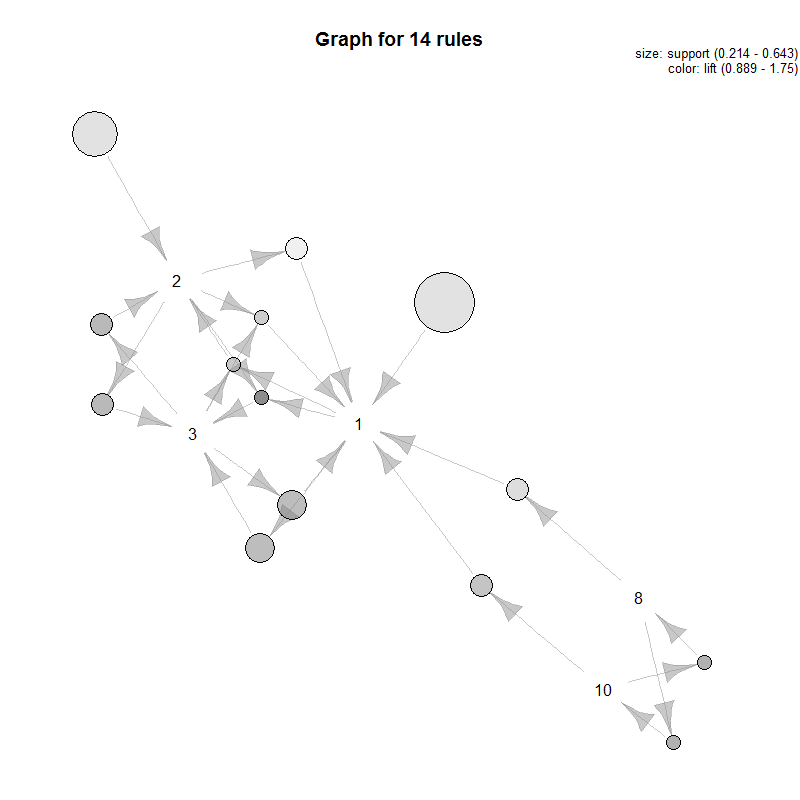
\includegraphics[scale=0.5]{associationbyfilm_1.png}\\
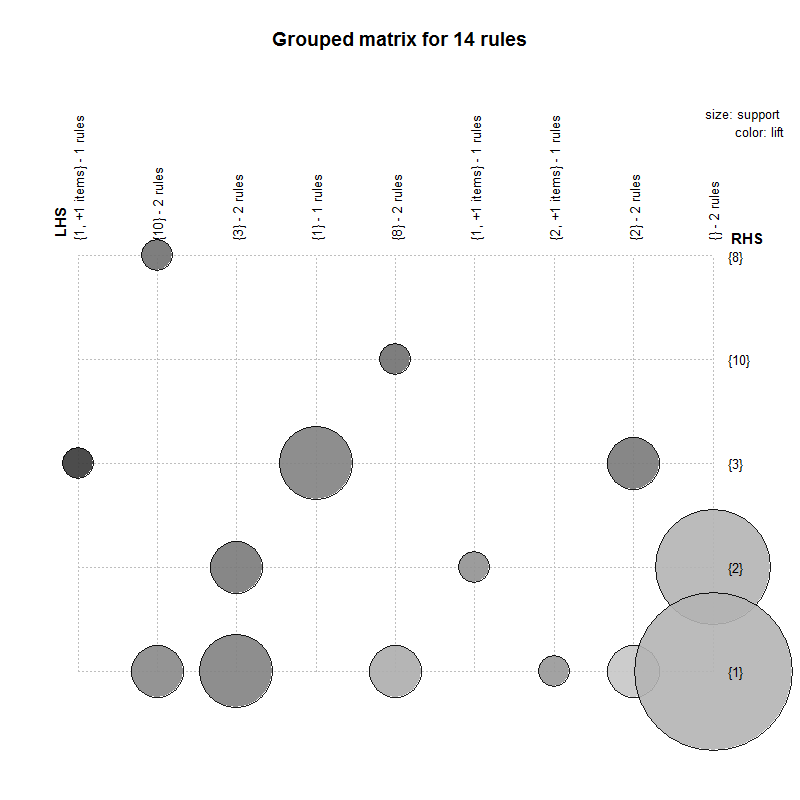
\includegraphics[scale=0.5]{associationrulebyfilm_2.png}\\
\end{enumerate}
\end{enumerate}
\subsection{Knn Neighbors}
K-Nearest neibhour is used for selection problem. It selects the most probable item which is similar to the test dataset.\\
Here the input dataset/train dataset is the dataframe of customers as columns and films as rows. package class is used for KNN neibhour algorithm.
\begin{enumerate}
\item Program:\\
The code of KNN is fairly simple. The entire dataframe other than the labels form training dataset. The data to be predicted for is the nearest neighbor of films 2,5,8,9 which is made as training set. The k nearest elements were chosen to be 3.\\
\lstinputlisting[language=R]{knn.R}

This algorithm was run multiple times. There were different outputs every time.\\
The most consistent result seems to be 14 out of few tests.\\
\begin{verbatim}
[1] CID5
Levels: CID1 CID10 CID11 CID12 CID13 CID14 CID2 CID3 CID4 CID5 CID6 CID7 CID8 CID9
> ru_knn<-knn(movie_df[-1],movie_test[,-1],movie_df[,1],k=3)
> ru_knn
[1] CID14
Levels: CID1 CID10 CID11 CID12 CID13 CID14 CID2 CID3 CID4 CID5 CID6 CID7 CID8 CID9
> ru_knn<-knn(movie_df[-1],movie_test[,-1],movie_df[,1],k=3)
> ru_knn
[1] CID14
Levels: CID1 CID10 CID11 CID12 CID13 CID14 CID2 CID3 CID4 CID5 CID6 CID7 CID8 CID9
\end{verbatim}
Hence the most nearest similar customer who has seen 2,5,8,7 is customer 14.
\end{enumerate}
\subsection{Naive Bayes}
Following is the code written for naive bayes implementation.
\lstinputlisting[language=R]{nbayes.R}
The output is given was movie 2.
\subsection{Agglomerative Hierarchial Clustering}
Inorder to find how the genre are related to teach other, we take up the transpose of the customer vs genere dataset.\\
The distance is calculated between these items in this dataset and is passed as parameter to the hclust algorithm.\\
The Datase Structure is as follows,
\begin{verbatim}
           V1 V2 V3 V4 V5 V6 V7 V8 V9 V10 V11 V12 V13 V14
Romance      5  0  3  2  2  2  1  2  0   2   2   1   2   2
SciFi        1  2  1  1  1  0  2  1  0   1   2   1   2   1
Horror       2  1  1  1  1  1  1  1  0   1   1   1   0   0
Comedy       2  2  1  1  1  0  1  1  0   1   2   1   0   1
Drama        3  3  0  2  1  1  1  1  0   0   2   1   3   0
Action       2  3  0  2  1  2  2  1  1   1   0   1   3   1
Documentary  0  3  0  1  1  1  2  1  1   1   0   1   1   1
Classic      1  2  1  1  1  2  2  1  1   2   0   1   1   1

>d
             Romance    SciFi   Horror   Comedy    Drama   Action Documentary
SciFi       5.830952                                                         
Horror      5.291503 3.162278                                                
Comedy      5.477226 2.449490 2.000000                                       
Drama       5.830952 3.464102 4.242641 4.000000                              
Action      6.164414 3.741657 4.472136 4.690416 3.162278                     
Documentary 7.483315 3.162278 3.741657 3.741657 4.690416 3.162278            
Classic     5.916080 3.316625 3.000000 3.605551 4.795832 3.000000    2.236068
\end{verbatim}
This data is then plotted with method average and ward.D method.\\
Code:\\
\lstinputlisting[language=R]{dendogram.R}
\begin{enumerate}
\item Ward.D :\\
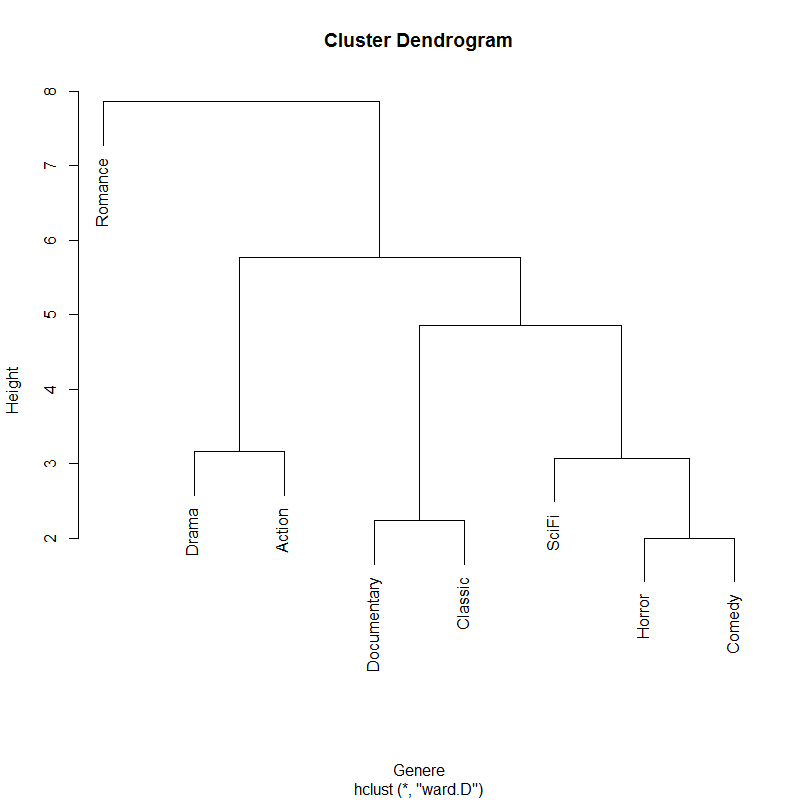
\includegraphics[scale=0.5]{hierarchial1.png}\\
\item Un Weighted Average:\\
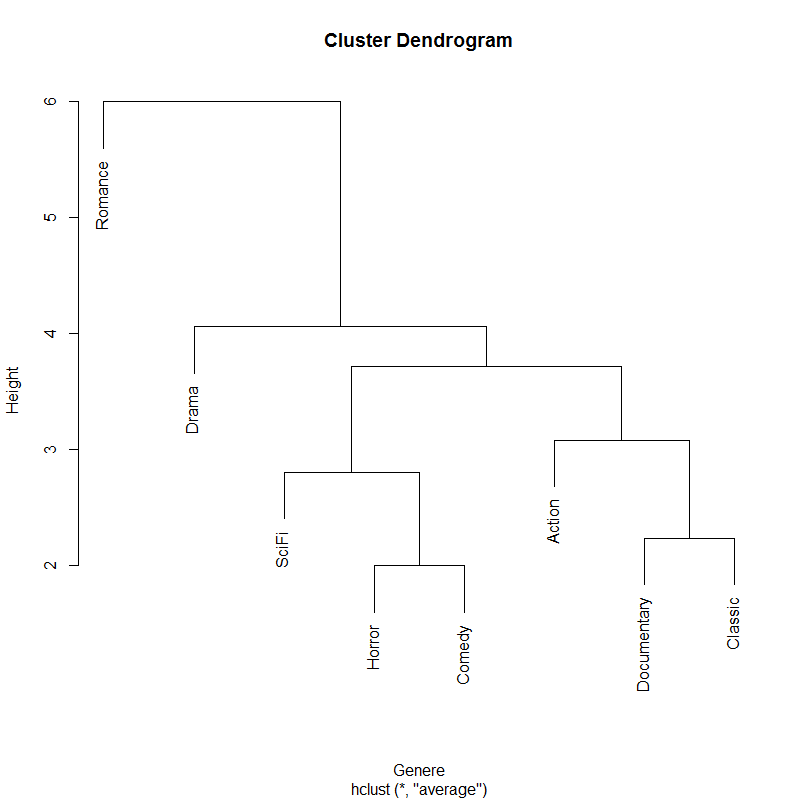
\includegraphics[scale=0.5]{dendogram_2.png}\\
\end{enumerate}
Both clusters represent similar things.\\
With respect to average cluster method,\\
People usually see Documentary and Classic together. \\
People who see Documentary and classic also see Action movies.\\
Hence rest of the plot can be interpreted as such.
\section*{Equivocation of k-l means algorithm}
\subsection*{Algorithm}
\begin{center}
\begin{algorithmic}[1]\label{k,l-means}
\State{\bf ALGORITHM} \texttt{k,l-means}
\State {\bf INPUT} (\textsf{data} $\Delta$, distance $d:\Delta^2\rightarrow \mathbb{R}_{\geq 0}$, \textsf{centoid number} $k$, \textsf{Closest Matches} $\ell$, \textsf{threshold} $\tau$)
\State {\bf OUTPUT} (\textsf{Set of centoids} $c_1, c_2, \ldots, c_k$)
\State Assume centroid is structure $c = (v \in DOM(\Delta), B\subseteq \Delta)$
\State  $c.v$ is the centroid value and $c.B$ is the set of nearest points.
\State $\tau$ is a percentage change from previous centroids
\State For example, $\{c_1, c_2, \ldots, c_k\}$ is previous and $\{d_1, d_2, \ldots, d_k\}$ is current
\State Total difference is $\Sigma_i \Sigma_j d(c_i, d_j)$
\State $Dom(\Delta)$ denotes domain of object.
\State $i = 0$
\Comment{Initialize iterate where superscript is iteration}
\For{$j = 1,k$}
\Comment{Initialize Centroids}
\State $c_j^i.v \gets  random(Dom(\Delta))$
\State $c_j^i.B \gets \emptyset$
\EndFor
\State $f_i = \Sigma_{j=1}^k\Sigma_{\ell = 1}^k d(c_j^i.v, random(Dom(\Delta))$
\Comment{Bootstrap difference between past centroids and current}
\Repeat
\color{blue}
\State $i \gets i + 1$
\For {$\delta \in \Delta$}
\For {$k=0; k< l; k++$}
\State $c_j^i.B \gets c.B \cup \{\delta\}$, where $\min_{c_j^i}\{d(\delta, c_j^i.v)\}$
\State \Comment{Associate a data point $\delta$ with the nearest l $c_j^i.v$}
\State Replace $\min_{c_j^i}\{d(\delta, c_j^i.v)\} $ with $ \max_{c_j^i}\{d(\delta, c_j^i.v)\}+1$
\State \Comment{This step is done so that the same minimum distance is not considered during other iteration}
\EndFor
\EndFor
\For {$j = 1, k$}
\State $c_j^i.v \gets ave(c_j^i.B)$
\Comment{Update centroid to be {\it best} representative of nearest data}
\State $c_j^i.B \gets \emptyset$
\Comment{$ave$ is easiest representative}
\EndFor
\color{black}
\Until{$(|f_i - f_{i-1}| < \tau(f_{i-1}))$}
\State {\bf return} ($c_1^i, c_2^i, \ldots, c_3^i$) 
\end{algorithmic}
\end{center}

\subsection*{Illustration}
\begin{enumerate}
\item Suppose [1 2 3 4 5] is a row in distance matrix corresponding to the datum n.\\
From the distance matrix, it can be inferred that there are 5 centroids. Consider l=2,
\begin{verbatim}
Iteration 1: [1 2 3 4 5] - Datum n is associated with centroid 1
Replace the distance : [6 2 3 4 5]
Iteration 2: [6 2 3 4 5] - Datum n is associated with centroid 2
Replace the distance : [6 7 3 4 5]
Iterations Reached l.
Datum point n is now associated with centroid 1 and 2
# Average and update the new representative.
\end{verbatim}
\item Java Implementation
\begin{enumerate}
\item
\begin{verbatim}
for(int j=0;j<l;j++){
	int noP=kCentroids_l.get(tuple_l.indexOf(Collections.min(tuple_l))).noPoints;
	kCentroids_l.get(tuple_l.indexOf(Collections.min(tuple_l))).intIndex[noP]=i;
	kCentroids_l.get(tuple_l.indexOf(Collections.min(tuple_l))).currPoints[noP]=(int)dataSet.get(i, 0);
	kCentroids_l.get(tuple_l.indexOf(Collections.min(tuple_l))).noPoints++;
	tuple_l.set(tuple_l.indexOf(Collections.min(tuple_l)),Collections.max(tuple_l)+1);
		}
\end{verbatim}
\item DataStructure Framework: EJML, Efficient Java Matrix Library is an open source library for extending matrix data structures to java. This supports loading of CSV files directly as matrix, perform advanced operations like matrix, SVD, and calculate distances. However for the purpose of this assignment, they are just used as data structures and this assignment uses no advanced operation required of these data structures.
\item Data munging for EJML : EJML reads data only as matrix and requires space separation instead of comma separated values. Hence these steps are done manually to replace comma with a space and replace first line with number of rows, columns and the data type. Following is a sneak peak of the file used for this assignment.
\begin{verbatim}
683 11 real
1000025 5 1 1 1 2 1 3 1 1 2
1002945 5 4 4 5 7 10 3 2 1 2
1015425 3 1 1 1 2 2 3 1 1 2
1016277 6 8 8 1 3 4 3 7 1 2
1017023 4 1 1 3 2 1 3 1 1 2
1017122 8 10 10 8 7 10 9 7 1 4

\end{verbatim}
\item Program Invocation: The program takes 7 parameters, input file, distance function, number of clusters, number of iterations, tolerance, featurset and l. Feature set is an comma separated string which contains index of strings that are to be considered for the clustering. This is useful when we can select only few features as predictor values rather than the entire attribute set. Following is the signature used to execute the data analysis. Currently only Eucledian distance is supported. This rather an provision for further improvement.
\begin{verbatim}
"d:\\bcdata.csv" eucledian 2 5 0.1 1,2,3,4,5,6,7,8,9 2
\end{verbatim}
\item Interpreting the Results: Following is a snapshot of the output.
\begin{verbatim}
------------------------Iteration 2 ------------------------
Cluster Id : 0
Cluster Centers : Type = dense real , numRows = 1 , numCols = 11
1324572.000   7.167   6.744   6.709   5.684   5.449   7.850   6.056   6.017   2.560

Previous Centers : Type = dense real , numRows = 1 , numCols = 11
1324572.000   7.075   6.427   6.416   5.459   5.290   7.427   5.859   5.792   2.514

Cluster Points[1002945, 1016277, 1017122]
Cluster Internal Indexes[1, 3, 5, -1]

Cluster Id : 1
Cluster Centers : Type = dense real , numRows = 1 , numCols = 11
1347749.000   3.022   1.278   1.394   1.343   2.080   1.301   2.085   1.229   1.105  

Previous Centers : Type = dense real , numRows = 1 , numCols = 11
1347749.000   2.874   1.199   1.308   1.264   2.009   1.231   2.007   1.129   1.061  

Cluster Points[1000025, 1015425, 1017023, 841769]
Cluster Internal Indexes[0, 2, 4, 6, 7, -1]

------------------------Has Converged : Tolerance------------------------
\end{verbatim}
The above is a snapshot of the output. There is an iteration number associated with these centroids. There are current centers and previous centers for every centroid. There is also references to data points associated to that centroid and reference to index of the data points. Also it gives details about if the convergence was by tolerance or iteration.
\item Application Design: The application mainly consists of two classes, Centroid and kMeans. Centroid class is mainly used as a integrated data structure encompassing multiple array vectors and matrices for holding statuses, values and to holding centroids. the driver class consists of modular functions for processing these centroid objects. These centroids are passes as array of objects using Java Collection framework. It has modular functions for reassigning centroid, calculating distances etc.
\end{enumerate}
\item Running the Program for l=2
\begin{verbatim}
Features Considered are[1, 2, 3, 4, 5, 6, 7, 8, 9]

------------------------Iteration 1 ------------------------
Cluster Id : 0
Cluster Centers : Type = dense real , numRows = 1 , numCols = 11
1148278.000   4.442   3.151   3.215   2.830   3.234   3.545   3.445   2.870   1.603   4.000  

Previous Centers : Type = dense real , numRows = 1 , numCols = 11
1148278.000   4.442   3.151   3.215   2.830   3.234   3.545   3.445   2.870   1.603   4.000  

Cluster Points[1000025, 1002945, ...897471]
Cluster Internal Indexes[0, 1, ... -1]

Cluster Id : 1
Cluster Centers : Type = dense real , numRows = 1 , numCols = 11
1336798.000   4.442   3.151   3.215   2.830   3.234   3.545   3.445   2.870   1.603   2.000  

Previous Centers : Type = dense real , numRows = 1 , numCols = 11
1336798.000   4.442   3.151   3.215   2.830   3.234   3.545   3.445   2.870   1.603   2.000  

Cluster Points[1000025, 1002945, ... 897471]
Cluster Internal Indexes[0, 1, .. -1]

------------------------Has Converged : Tolerance------------------------
\end{verbatim}
When the program was run for the breast cancer dataset, with centroids =2 and l=2, it was seen that all centroids had all points, which is expected since there are only two centroids and all points are associated with two centroids.\\ \\
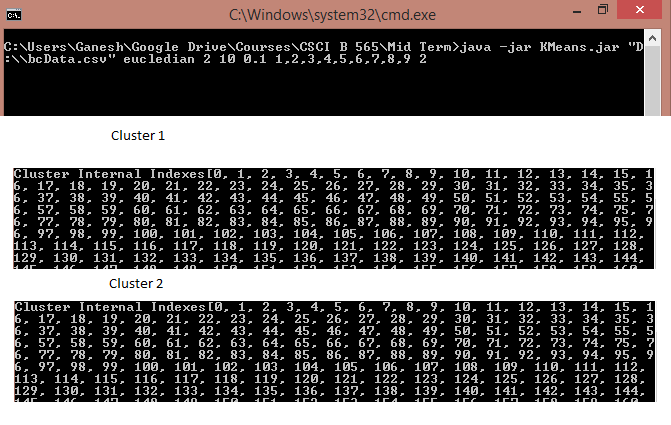
\includegraphics[scale=0.7]{kmeansStart.png}\\
\end{enumerate}
\section*{Statistical Dependency and Correlation}
\subsection{Problem Statement}
Given two columns which can take only following values (Yes, No), (No, Yes) and (Maybe, No).\\
\begin{enumerate}
\item Statistical Dependency:
\begin{enumerate}
\item Consider X and Y be the random variables over the probability distribution of columns Do you own a house? and Do you own a car. These random variables are said to be dependent only when X is a linear/non-linear function of Y.
\item It is given that instead of all possible values, X and Y can only take few set of discrete values, ie (Yes, No), (No, Yes) and (Maybe, No), ie when X is Yes, Y must be NO. The similar inference can be done for other two cases.
\item It can be also noted that there cannot be any value which is (Yes, Yes) or (No,No) , ie no probabilistic independence, hence Random variables X and Y are dependent.
\item Hence from the above discussion, Both the columns are statistically dependent.
\end{enumerate}
\item Statistical Correlation:
\begin{enumerate}
\item Assuming when two random variables X and Y are dependent, statistical correlation gives the expectation of a Random variable Y given X.
\item E.g, from the given data, converting the categorical values to nominal values, Yes = 1, No = 0, MayBe = 0.5. Also considering that all these three are in same proportion, following R code gives the correlation.
\begin{verbatim}
> cor(cbind(c(1,0,0.5),c(0,1,0)))
           [,1]       [,2]
[1,]  1.0000000 -0.8660254
[2,] -0.8660254  1.0000000
> cor(cbind(c(1,0,0.5,1,0,0.5),c(0,1,0,0,1,0)))
           [,1]       [,2]
[1,]  1.0000000 -0.8660254
[2,] -0.8660254  1.0000000
\end{verbatim}
\item Since when there is X=1, Y=0, and Y=1 and X=0, There is a negative corrleation as suggested by the 
\end{enumerate}
\end{enumerate}
\section*{References and Acknowlegements}
Following links were referred for this assignment
\begin{enumerate}
\item http://stackoverflow.com/questions/16515370/r-basket-analysis-using-arules-package-with-unique-order-number-but-duplicate-or
\item https://prdeepakbabu.wordpress.com/2010/11/13/market-basket-analysisassociation-rule-mining-using-r-package-arules/
\item http://stats.stackexchange.com/questions/31083/how-to-produce-a-pretty-plot-of-the-results-of-k-means-cluster-analysis
\item http://stackoverflow.com/questions/12911234/clustering-large-data-matrix-using-r
\item http://www.rdatamining.com/examples/association-rules
\item http://www.rdatamining.com/docs/data-clustering-with-r
\item http://stackoverflow.com/questions/6750546/export-csv-without-col-names
\item http://stackoverflow.com/questions/32449280/how-to-create-a-decision-boundary-graph-for-knn-models-in-the-caret-package
\item http://blog.datacamp.com/machine-learning-in-r/
\item http://www.statmethods.net/advstats/cluster.html
\item http://stackoverflow.com/questions/32677141/how-to-plot-using-ggplot2-a-numeric-variable-against-categorical-variable-after
\item Peter Abeles, and Institute for Human Machine Cognition for EJML library
\end{enumerate}
\end{document}
